\documentclass{article}
\usepackage{amsmath}
\usepackage{titlesec}
\usepackage[mathletters]{ucs}
\usepackage[utf8x]{inputenc}
\usepackage[margin=1.5in]{geometry}
\usepackage{enumerate}
\newtheorem{theorem}{Theorem}
\usepackage[dvipsnames]{xcolor}
\usepackage{pgfplots}
\pgfplotsset{compat=1.18}
\setlength{\parindent}{0cm}
\usepackage{graphics}
\usepackage{graphicx} % Required for including images
\usepackage{subcaption}
\usepackage{bigintcalc}
\usepackage{pythonhighlight} %for pythonkode \begin{python}   \end{python}
\usepackage{appendix}
\usepackage{arydshln}
\usepackage{physics}
\usepackage{booktabs} 
\usepackage{adjustbox}
\usepackage{mdframed}
\usepackage{relsize}
\usepackage{physics}
\usepackage[thinc]{esdiff}
\usepackage{esint}  %for lukket-linje-integral
\usepackage{xfrac} %for sfrac
\usepackage{hyperref} %for linker, må ha med hypersetup
\usepackage[noabbrev, nameinlink]{cleveref} % to be loaded after hyperref
\usepackage{amssymb} %\mathbb{R} for reelle tall, \mathcal{B} for "matte"-font
\usepackage{listings} %for kode/lstlisting
\usepackage{verbatim}
\usepackage{graphicx,wrapfig,lipsum,caption} %for wrapping av bilder
\usepackage{mathtools} %for \abs{x}
\usepackage[english]{babel}
\usepackage{cancel}
\definecolor{codegreen}{rgb}{0,0.6,0}
\definecolor{codegray}{rgb}{0.5,0.5,0.5}
\definecolor{codepurple}{rgb}{0.58,0,0.82}
\definecolor{backcolour}{rgb}{0.95,0.95,0.92}
\lstdefinestyle{mystyle}{
    backgroundcolor=\color{backcolour},   
    commentstyle=\color{codegreen},
    keywordstyle=\color{magenta},
    numberstyle=\tiny\color{codegray},
    stringstyle=\color{codepurple},
    basicstyle=\ttfamily\footnotesize,
    breakatwhitespace=false,         
    breaklines=true,                 
    captionpos=b,                    
    keepspaces=true,                 
    numbers=left,                    
    numbersep=5pt,                  
    showspaces=false,                
    showstringspaces=false,
    showtabs=false,                  
    tabsize=2
}

\lstset{style=mystyle}
\author{Oskar Idland}
\title{Oblig 4}
\date{}
\begin{document}
\maketitle
%\tableofcontents
\newpage

\section*{Problem 1}
\subsection*{a)}
\begin{figure}[h!]
\centering
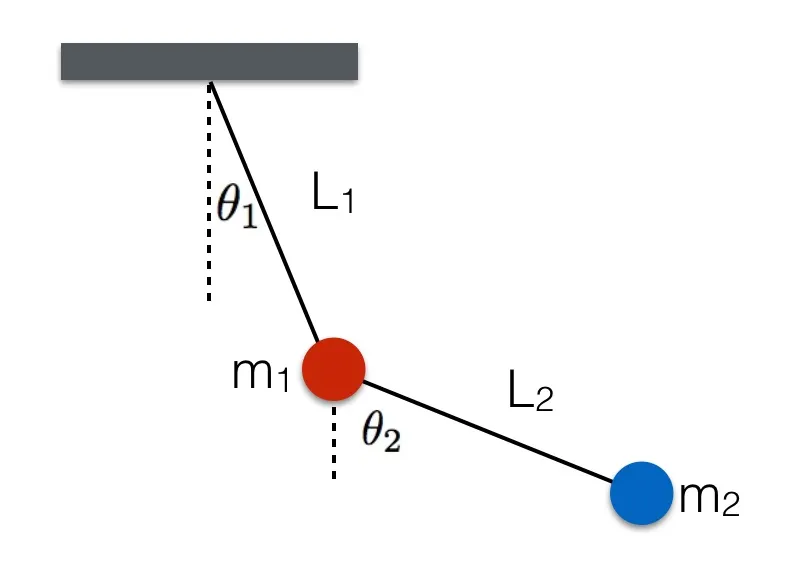
\includegraphics[width = \textwidth]{DoublePendulum.png}
\caption{Scheme of the double pendulum. We have two bodies with masses $m_1$ and $m_2$, and lengths $l_1$ and $l_2$ respectively. The angles are $θ_1$ and $θ_2$.}
\label{fig: 1a}
\end{figure}

We have 2 bodies in 2 dimensions with 2 constraints ($l_1$ and $l_2$). This gives:
\[
d = 2 ⋅ 2 - 2 = 2
\]
We get the following coordinates:
\[
\underline{\underline{q_1 = θ_1 \quad , \quad  q_2 = θ_2}}
\]

\subsection*{b)}
We use the lengths and angles to find the $x$ and $y$ coordinates of the two bodies. We get:
\[
x_1 = l_1 \sin θ_1 \quad  \ \ \ , \quad y_1 = -l_1 \cos θ_1
\]
\[
x_2 = l_1 \sin θ_1 + l_2 \sin θ_2 \quad \ \ \ , \quad y_2 = -l_1 \cos θ_1 - l_2 \cos θ_2
\]
\[
\dot{x}_1 = l_1 \dot{θ}_1 \cos θ_1 \quad , \quad \dot{y}_1 = l_1 \dot{θ}_1 \sin θ_1
\]
\[
\dot{x}_2 = l_1 \dot{θ}_1 \cos θ_1 + l_2 \dot{θ}_2 \cos θ_2 \quad , \quad \dot{y}_2 = l_1 \dot{θ}_1 \sin θ_1 + l_2 \dot{θ}_2 \sin θ_2
\]
Then we just insert these into the formula for kinetic and potential energy: 
\[
T = \frac{1}{2}m_1 v_1^2 + \frac{1}{2}m_2 v_2^2
\]
\[
T = \frac{1}{2} m_1 \left( \dot{x}_1^2 + \dot{y}_1^2 \right) + \frac{1}{2} m_2 \left( \dot{x}_2^2 + \dot{y}_2^2 \right)
\]
\begin{align*}
T = &\frac{1}{2} m_1 \left( \left( l_1 \dot{θ}_1 \cos θ_1 \right)^2 + \left( l_1 \dot{θ}_1 \sin θ_1 \right)^2 \right) + \\ &\frac{1}{2} m_2 \left( \left( l_1 \dot{θ}_1 \cos θ_1 + l_2 \dot{θ}_2 \cos θ_2 \right)^2 + \left( l_1 \dot{θ}_1 \sin θ_1 + l_2 \dot{θ}_2 \sin θ_2 \right)^2 \right)
\end{align*}
Using this trig identity:
\[
\cos θ_1 \cos θ_2 + \sin θ_1 \sin θ_2 = \cos(θ_1 - θ_2)
\]
We get the following:
\[
T = \underline{\underline{\frac{1}{2}m_1l_1^2\dot{θ}_1^2 + \frac{1}{2}m_2\left(l_1^2\dot{θ}_1^2 + l_2^2\dot{θ}_2^2 + 2l_1l_2\dot{θ}_1\dot{θ}_2\cos(θ_1 - θ_2)\right)}}
\]
\[
V = m_1 g y_1 + m_2 g y_2
\]
\[
V = m_1 g (-l_1 \cos θ_1) + m_2 g (-l_1 \cos θ_1 - l_2 \cos θ_2)
\]
\[
V = \underline{\underline{-(m_1 + m_2) g l_1 \cos θ_1 - m_2 g l_2 \cos θ_2}}
\]

Putting everything together we get the Lagrangian $L$:
\[
L = T - V
\]
\begin{align*}
L = &\frac{1}{2} m_1 \left( \left( l_1 \dot{θ}_1 \cos θ_1 \right)^2 + \left( l_1 \dot{θ}_1 \sin θ_1 \right)^2 \right) + \\ &\frac{1}{2} m_2 \left( \left( l_1 \dot{θ}_1 \cos θ_1 + l_2 \dot{θ}_2 \cos θ_2 \right)^2 + \left( l_1 \dot{θ}_1 \sin θ_1 + l_2 \dot{θ}_2 \sin θ_2 \right)^2 \right) \\ &+(m_1 + m_2) g l_1 \cos θ_1 + m_2 g l_2 \cos θ_2
\end{align*}

\subsection*{c)}
Beginning with the canonical momentum $p$:
\[
p_{θ_1} = \frac{∂ L}{∂ \dot{θ}_1} = \frac{∂ T}{∂ \dot{θ}_1} = (m_1 + m_2) l_1^2 \dot{θ}_1 + m_2 l_1 l_2 \dot{θ}_2 \cos(θ_1 - θ_2)
\]
\[
p_{θ_2} = \frac{∂ L}{∂ \dot{θ}_2} = \frac{∂ T}{∂ \dot{θ}_2} = m_2 l_2^2 \dot{θ}_2 + m_2 l_1 l_2 \dot{θ}_1 \cos(θ_1 - θ_2) 
\]
Now we can find the equations of motion:
\[
\frac{∂ p_{θ_1}}{∂ t} - \frac{∂ L}{∂ θ_1} = 0
\]
\begin{align*}
\frac{∂ p_{θ_1}}{∂ t} = &(m_1 + m_2) l_1^2 \ddot{θ}_1 + m_2 l_1 l_2 \ddot{θ}_2 \cos(θ_1 - θ_2)\\ &- m_2 l_1 l_2 \dot{θ}_2 \dot{θ}_1 \sin(θ_1 - θ_2) + m_2 l_1 l_2 \dot{θ}_2^2 \sin(θ_1 - θ_2)
\end{align*}

\begin{align*}
\frac{∂ L}{∂ θ_1} = -m_2l_1l_2\dot{θ}_1\dot{θ}_2\sin(θ_1 - θ_2) - (m_1 + m_2)gl_1\sin θ_1
\end{align*}

\begin{align*}
\frac{∂ p_{θ_2}}{∂ t} = &m_2 l_2^2 \ddot{θ}_2 + m_2 l_1 l_2 \ddot{θ}_1 \cos(θ_1 - θ_2)\\ &- m_2 l_1 l_2 \dot{θ}_1^2 \sin(θ_1 - θ_2) + m_2 l_1 l_2 \dot{θ}_1 \dot{θ}_2 \sin(θ_1 - θ_2)
\end{align*}

\begin{align*}
\frac{∂ L}{∂ θ_2} = m_2l_1l_2\dot{θ}_1\dot{θ}_2\sin(θ_1 - θ_2) - m_2gl_2\sin θ_2
\end{align*}

Now we can define the angles $θ_1$ and $θ_2$:
\begin{align*}
θ_1 = \underline{\underline{(m_1 + m_2)l_1 \ddot{θ}_1 + m_2 l_2 \ddot{θ}_2 \cos(θ_1 - θ_2)   + m_2 l_2 \dot{θ}_2^2 \sin(θ_1 - θ_2) + (m_1 + m_2) g \sin θ_1 = 0}}
\end{align*}

\begin{align*}
θ_2 = \underline{\underline{l_2\ddot{θ}_2 + l_1 \ddot{θ}_1 \cos(θ_1 - θ_2) - l_1 \dot{θ}_1^2 \sin(θ_1 - θ_2) + g \sin θ_2 = 0}}
\end{align*}

\subsection*{d)}
\begin{align*}
(m_1 + m_2) l_1 \ddot{θ}_1 &= -m_2l_2\ddot{θ}_2\cos(θ_1 - θ_2) \\ &- m_2l_2\dot{θ}_2^2\sin(θ_1 - θ_2) - (m_1 + m_2) g \sin θ_1
\end{align*}
\[
\ddot{θ} = \underline{\underline{ \frac{-m_2l_2\ddot{θ}_2\cos(θ_1 - θ_2) - m_2l_2\dot{θ}_2^2\sin(θ_1 - θ_2) - (m_1 + m_2) g \sin θ_1}{(m_1 + m_2) l_1}}}
\]
\[
l_2 \ddot{θ}_2 = l_1 \dot{θ}_1^2 \sin(θ_1 - θ_2) - g \sin θ_2 - l_1 \ddot{θ}_1 \cos(θ_1 - θ_2)
\]
\[
\ddot{θ}_2 = \underline{\underline{\frac{l_1 \dot{θ}_1^2 \sin(θ_1 - θ_2) - g \sin θ_2 - l_1 \ddot{θ}_1 \cos(θ_1 - θ_2)}{l_2}}}
\]


\section*{Problem 2}
\subsection*{a)}
\[
∂t = \frac{∂s}{v} \quad , \quad  v = \sqrt{-2gy} \quad , \quad  ∂s = \sqrt{\mathrm{d}x^2 + \mathrm{d}y^2}
\]
\[
y' = \frac{∂y}{∂x} 
\]
Simplifying the expression for $∂s$:
\[
∂s = \sqrt{1 + y'^2} \mathrm{d}x
\]
Finally we get the expression for $∂t$:
\[
∂t = \frac{\sqrt{1 + y'^2}}{\sqrt{-2gy}} \mathrm{d}x
\]
\[
∫_{0}^{T} ∂t = ∫_{x_{A}}^{x_{B}} \frac{\sqrt{1 + y'^2}}{\sqrt{-2gy}}  \ \mathrm{d}x
\]
\[
T (y(x)) = ∫_{x_{A}}^{x_{B}} \frac{\sqrt{1 + y'^2}}{\sqrt{-2gy}}  \ \mathrm{d}x = ∫_{v_{A}}^{v_{B}} L(y,y') \ \mathrm{d}x
\]

\subsection*{b)}
\[
H = p y' - L = \frac{∂ L}{∂ y'} y' - \sqrt{\frac{1 + y'^2}{-2gy}}
\]
\[
\underline{\underline{H = - \frac{1}{\sqrt{-2gy}(1 + y'^2)}}}
\]
The Hamiltonian is time independent, which means that it is a constant of motion. 

\[
- \frac{1}{\sqrt{-2gy}(1 + y'^2)} = C
\]
\[
 1 = C^2 (1 + y'^2) (-2gy)
\]
\[
\frac{1}{-2gC^2} = y(1 + y'^2)
\]
We define $k$ as the following:
\[
k = \sqrt{\frac{1}{2gC^2}}
\]
Giving:
\[
y(1 + y'^2) = -k^2
\]

\subsection*{c)}
\[
y' = \frac{∂y}{∂x} = \frac{∂y}{∂θ} = \frac{∂ θ }{∂ x} 
\]
\[
\frac{∂ x}{∂ θ} = \frac{1}{2} k^2 (1 - \cos θ) = -y
\]
\[
y' = \frac{∂ y}{∂ θ} \frac{1}{y}
\]
\[
(1+y'^2)y = \left(1 + \frac{1}{y^2} \left(\frac{∂ y}{∂ θ}^2\right)\right)y = \left(y^2 + \left(\frac{∂ y}{∂ θ}\right)^2\right) \frac{1}{y} = -k^2
\]
\[
\frac{∂ y}{∂ θ} = - \frac{k^2}{2} \sin θ
\]
\[
\left(y^2 + \left(\frac{∂ y}{∂ θ}\right)^2\right) \frac{1}{y} = \left(\left(\frac{1}{2} k^2 (\cos θ - 1)\right)^2 + \left(\frac{1}{2} k^2 \sin θ\right)^2\right) \frac{1}{y}
\]
\[
\left(y^2 \left(\frac{∂ y}{∂ θ}\right)^2\right) \frac{1}{y} = \frac{1}{4}k^{4} \left(\left(\cos θ - 1\right)^2 + \sin^2θ\right) \frac{1}{y}
\]
\[
\left(y^2 \left(\frac{∂ y}{∂ θ}\right)^2\right) \frac{1}{y} = \frac{1}{4}k^{4} \left(2 - 2\cos θ\right) \frac{1}{y}
\]
\[
\left(y^2 \left(\frac{∂ y}{∂ θ}\right)^2\right) = -k^2y \frac{1}{y} = -k^2
\]

\[
x_{A} = 0 → \frac{1}{2} k^2 (θ_{A} - \sin θ_{A}) = 0 → \underline{θ_{A} = 0}
\]
\[
y_{A} = 0 → \frac{1}{2} k^2 (\cos θ_{A} - 1) = 0 → \underline{θ_{A} = 2n\pi} \quad , \quad n \in \mathbb{Z}
\]
\[
x_{B} = \frac{1}{2} k^2 (θ_{B} - \sin θ_{B}) 
\]
\[
y_{B} = \frac{1}{2} k^2 (\cos θ_{B} - 1)
\]



\end{document}